\vspace{24pt}
\chapter{Исследование физических характеристик детектора <<Лазерного поляриметра>>}
\section{Определение уровня шумов детектора}
\label{sec:noise_study}
\begin{figure}[H]
	\begin{center}
		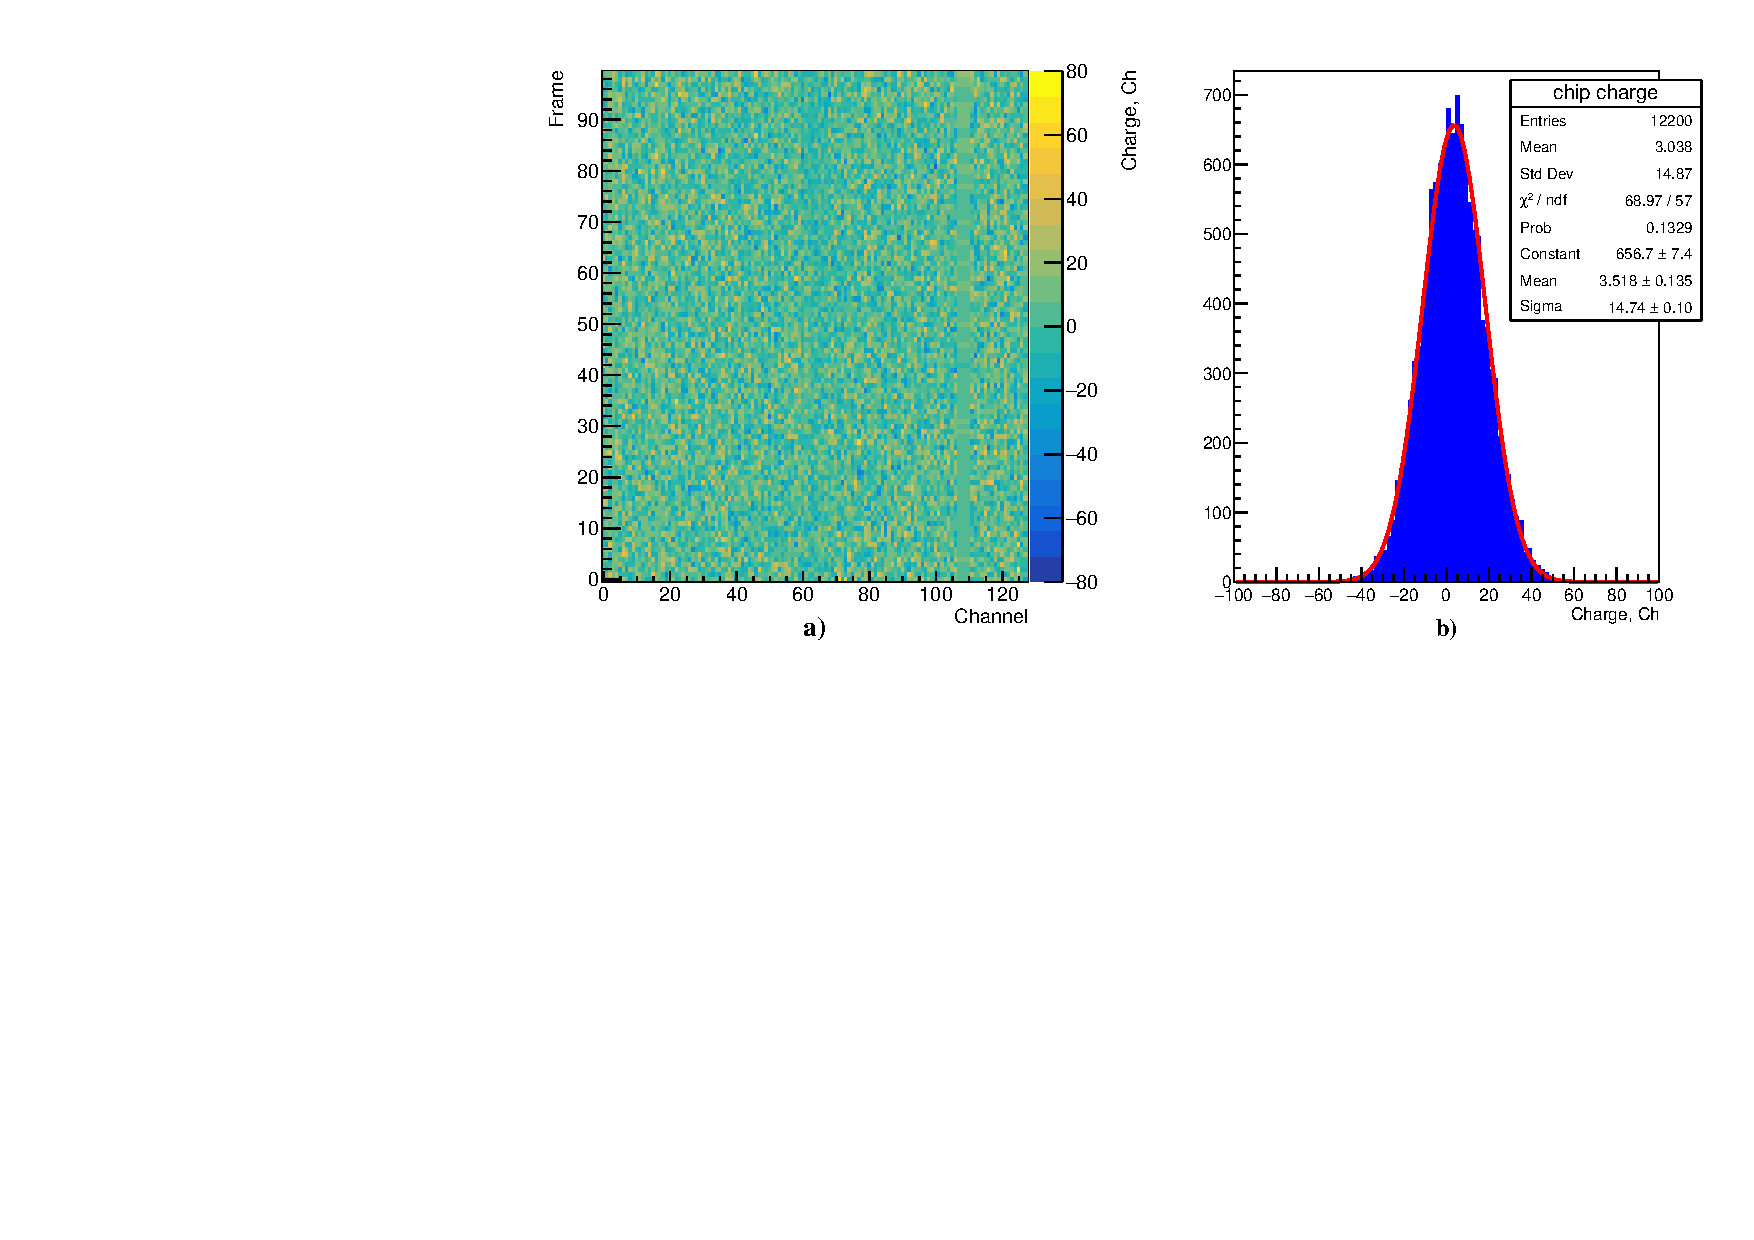
\includegraphics[width = 12cm, height = 6cm]{img/noise_map.pdf}
		\caption{a): Вид шумового события после вычитания пьедестала b): Распределение заряда в шумовом событии}
		\label{noise_map}
	\end{center}
\end{figure}
Рис. \ref{noise_map} показывает вид одного шумового события и распределение заряда в кадрах и каналах. Важным значением, которое можно извлечь уже из одного шумового события является уровень шумов. Его можно определить как корень из дисперсии распределения на Рис. \ref{noise_map} b). Шумы в данном эксперименте составили $\approx15$ каналов АЦП. Если взять несколько шумовых событий, то можно уточнить данное значение. Более того, записывая данные через равные промежутки времени, можно зафиксировать наличие дрейфа уровня шумов и их среднего значения. Такое исследование тоже было проведено. Для каждого набора данных существовала привязка по времени начала измерения. Чтобы определить, временной дрейф уровня среднего значения шумов, нами были Его результаты показали, что уровень шумов со временем меняется незначительно (Рис.\ref{fig:Noise_gr}.)

\begin{figure}[h]
	\centering
	\begin{subfigure}{.5\textwidth}
		\centering
		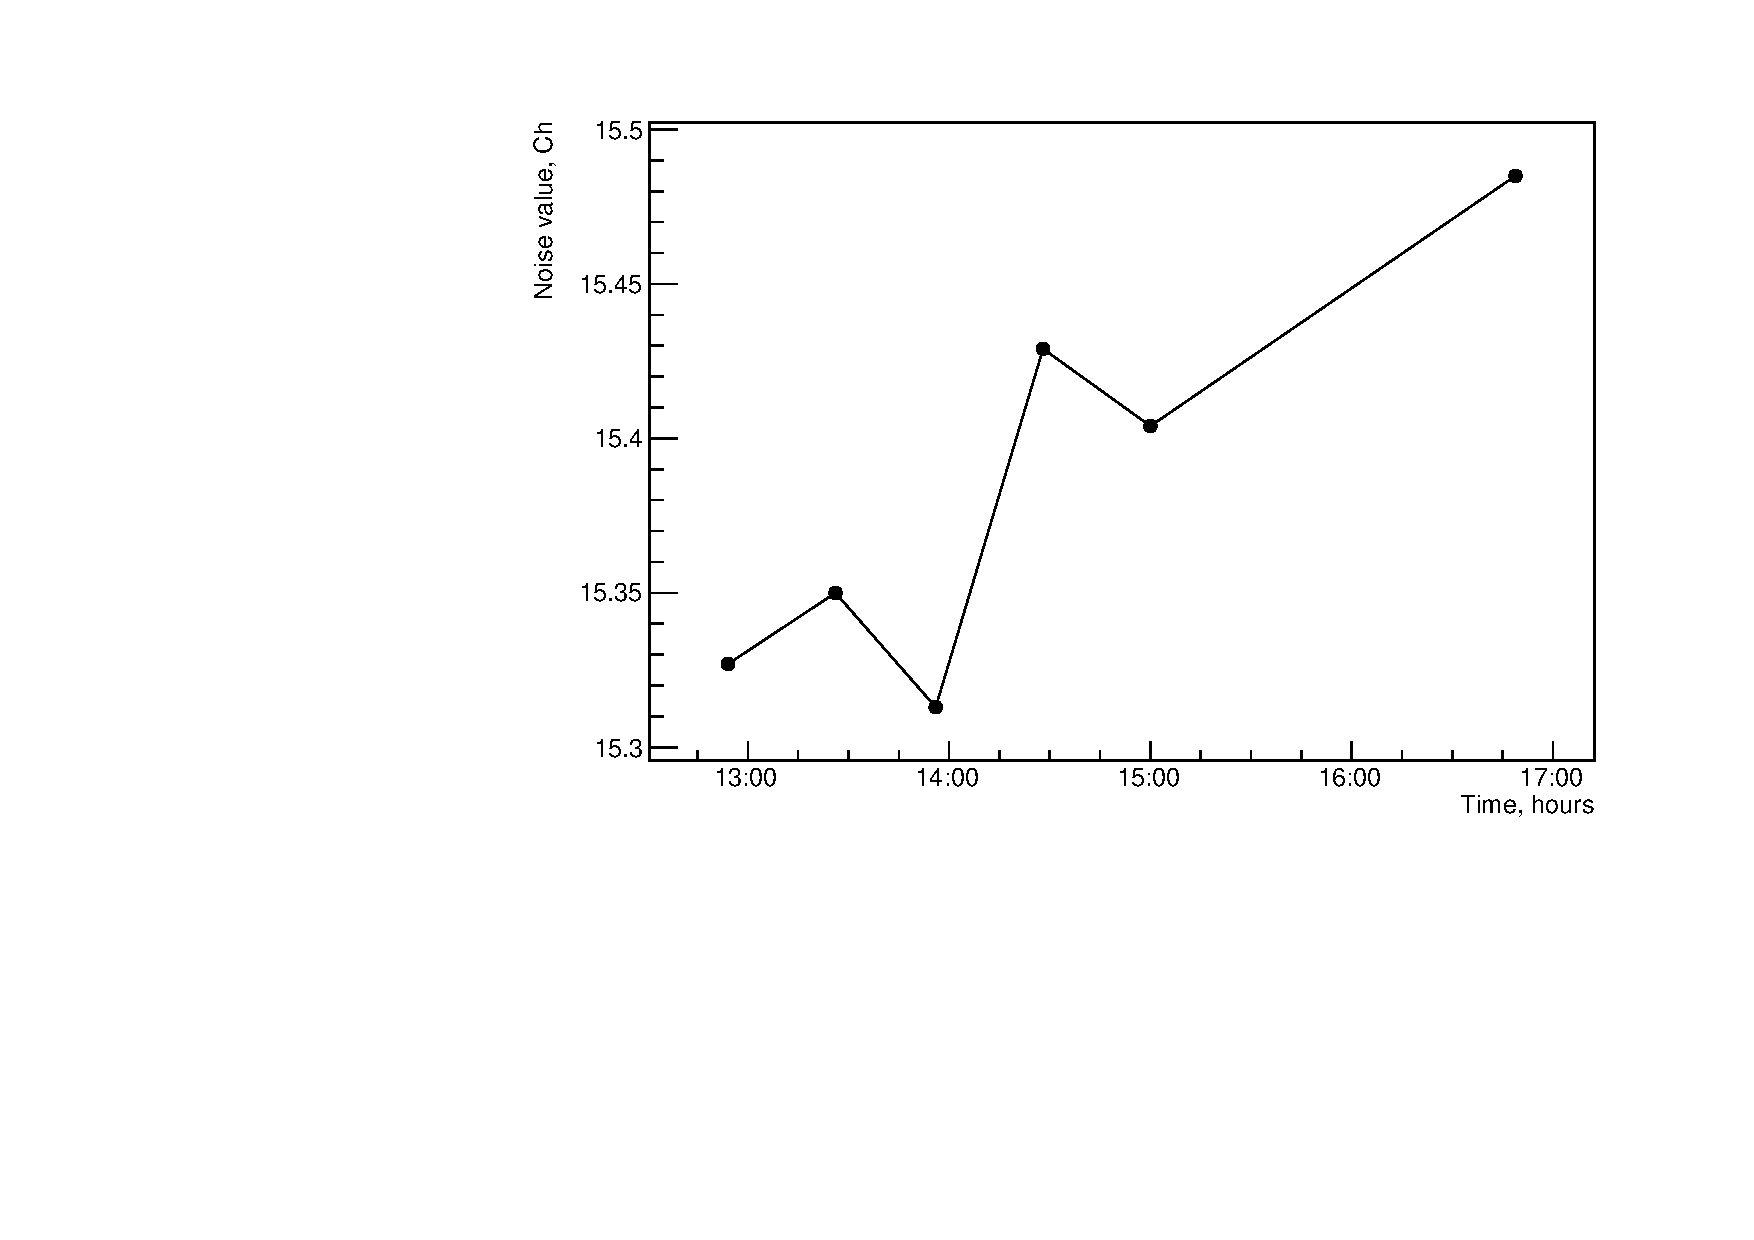
\includegraphics[width=1\linewidth]{img/Noise_time_drift.pdf}
		\caption{Уровень шумов}
	\end{subfigure}%
	\begin{subfigure}{.5\textwidth}
		\centering
		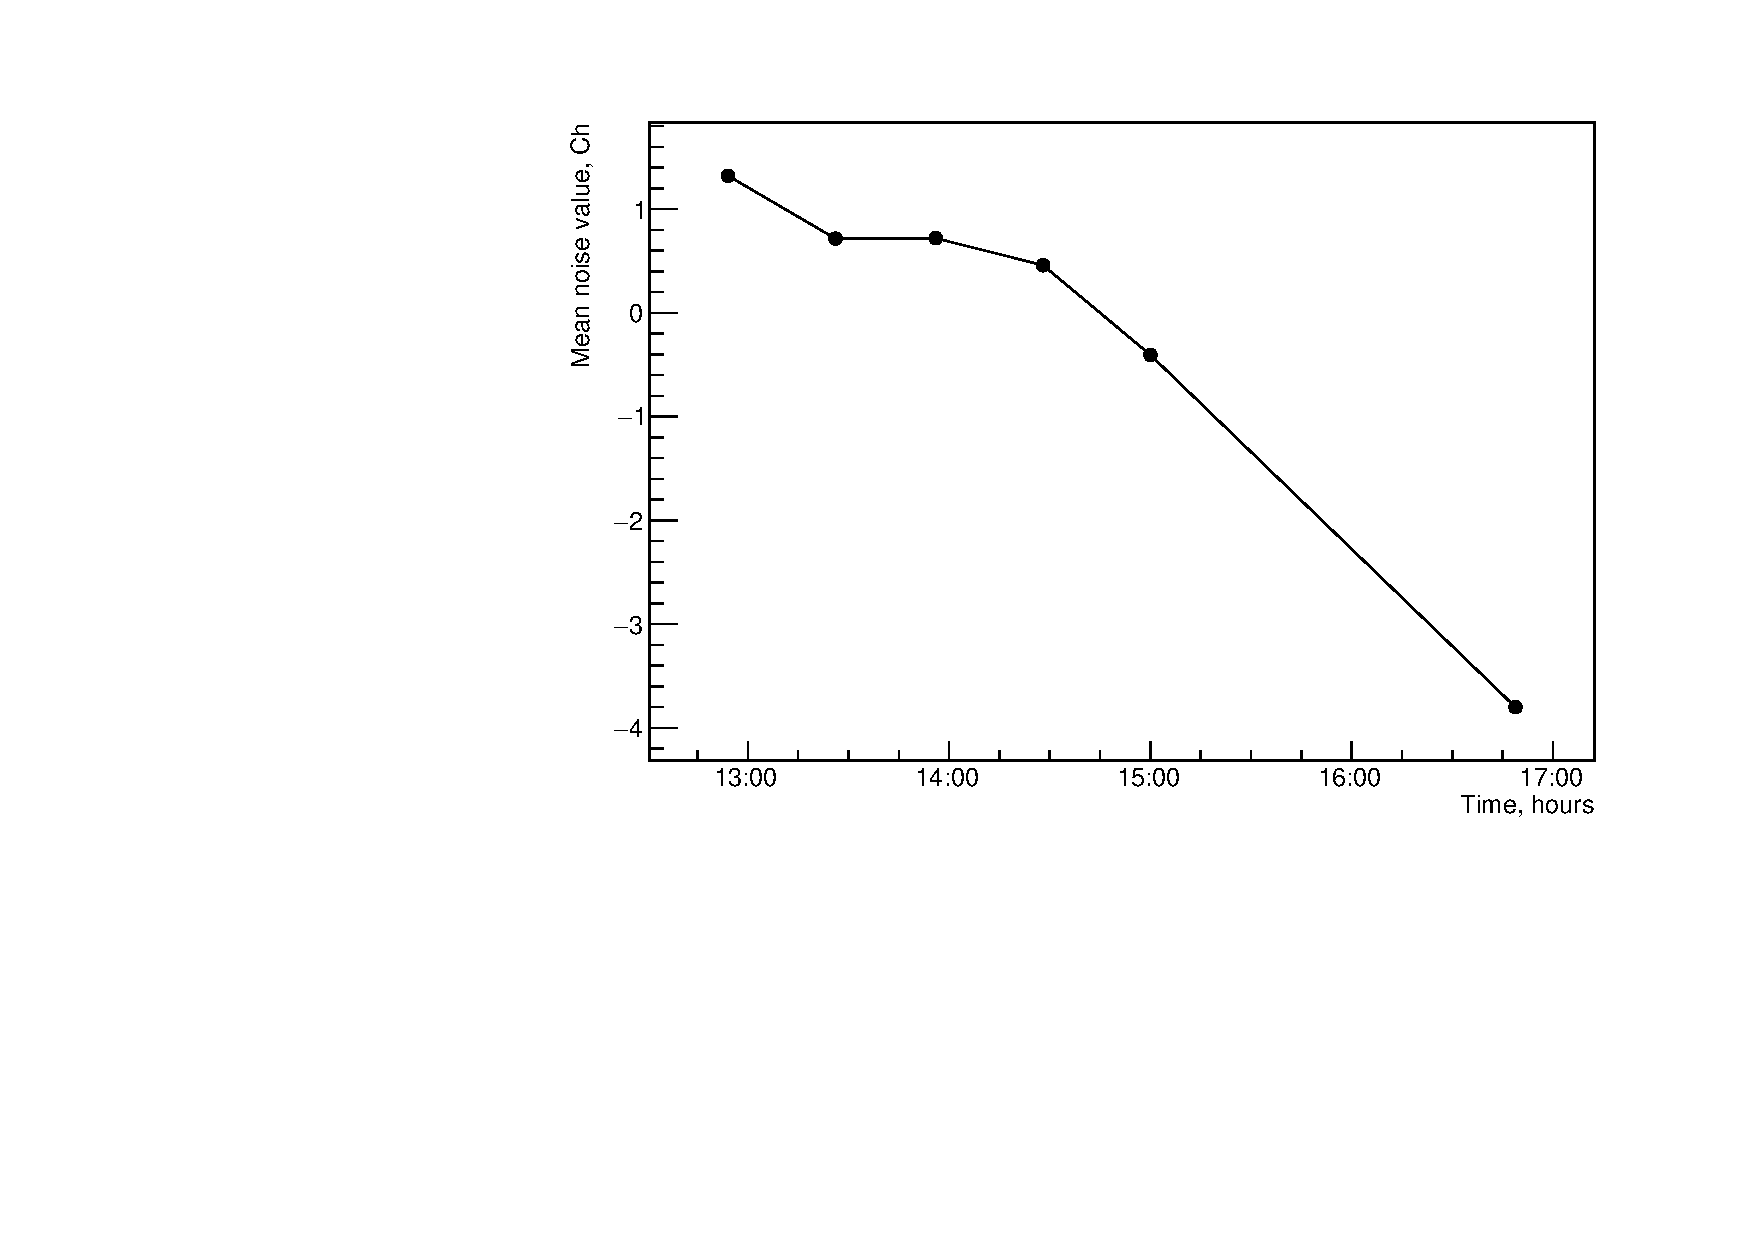
\includegraphics[width=1\linewidth]{img/Mean_time_drift.pdf}
		\caption{Среднее значение шума}
	\end{subfigure}
	\caption{Временной дрейф параметров шумовых событий: уровня шума и среднего значения шума. Каждая точка - среднее по $3\cdot10^7$ значений. В обоих случаях наблюдается линейный тренд. Статистические ошибки в точках малы и на графиках не видны}
	\label{fig:Noise_gr}
\end{figure}
Относительное изменение уровня шума за 4 часа составило $0.01~\sigma$, а дрейф среднего значения -- $0.33~\sigma$. Установившееся значение уровня шумов скорее всего зависит от температурного дрейфа электроники. Это является отдельной довольно обширной темой и в данной работе рассматриваться не будет. Однако, необходимы дополнительные долговременные эксперименты, которые смогут показать, каков максимально достижимый уровень шумов системы и насколько сдвигаются нулевые значения АЦП. Тем не менее, промежуточные результаты показали, что для <<Лазерного поляриметра>> это не является критичным.  
\section{Определение коэффициента усиления}
\label{sec:ampl_с}
При исследовании новой модели детектора необходимо различными методами проверить правильность работы, как ускоряющей структуры, так и вычитывающей электроники. Это можно сделать путём измерения коэффициента усиления детектора. 
%Стоит отметить, что зарегистрировать ионизацию первичной частицы достаточно сложно ввиду малого количества заряда. Для этого необходимы высокочувствительные АЦП. Однако, при использовании 
Коэффициент усиления в данной работе определяется как отношение зарегистрированного считывающей структурой заряда кластера к количеству частиц первичной ионизации, образованных в индукционном промежутке. 
Количество частиц первичной ионизации найдем, используя средние ионизационные потери и количество энергии, необходимое для образования ион--электронной пары. Известно, что потери энергии электронов в тонких слоях описываются модифицированной формулой Бете-Блоха:
\begin{equation}
\cfrac{dE}{dx} = \cfrac{2\pi N_0 e^4 Z\rho}{m_e c^2 \beta^2 A}\biggl[ln \bigg(\cfrac{ m_ec^2T\beta^2\gamma^2}{2I^2}\bigg) + f_{corr}(\beta)\biggr],
\label{eq:Bethe_Bloch}
\end{equation}
где $N_0$ -- число Авогадро, $e$ -- элементарный электрический заряд, $m_e$ -- масса электрона, $c$ -- скорость света, $\beta = v/c$ -- отношение скорости частицы к скорости света, $Z$ -- зарядовое число, $A$ -- массовое число, $\rho$ -- плотность вещества, $T$ -- кинетическая энергия электронов, $I$ -- энергия образования ион--электронной пары, $f_{coor}(\beta)$ -- функция, которая содержит поправки в случае $\beta \sim 1$. Параметры $A,Z,\rho$ относятся к веществу--радиатору т.е. к газовой смеси, которой заполнен детектор.
\par Вычисление показало, что средние потери энергии электронов с энергией $2.2~\MeV$ составляют $2.5~\keV/$см. Энергия образования одной ион--электронной пары в аргоне есть $26\eV$. Размер дрейфового промежутка -- 3 мм. Количество первичных электронов:
\begin{equation}
	N_e = \frac{dE/dx~\Delta x}{W} =\frac {2400~\eV/cm \cdot 0.3~cm}{26~\eV} = 28
\end{equation}
Зная средний заряд кластера $\langle Q\rangle$, можно определить коэффициент усиления системы GEM: 
\begin{equation}
K = \frac{\langle Q\rangle}{\langle N_e \rangle\ W},
\label{eq:ampl_k}
\end{equation}
где $I = 26~\eV$ -- средняя энергия образования ион-электронной пары в аргоне. 
\par Такой метод определения коэффициента усиления имеет один недостаток: в эксперименте определить средний заряд кластера достаточно трудно т.к. существуют ограничения электроники на максимальное измеренное значение. Более того, средний заряд кластера имеет распределение Ландау, параметром которого является наиболее вероятный заряд кластера. Поэтому вместо средних ионизационных потерь необходимо рассчитывать наиболее вероятные. Выражение для них можно записать следующим образом:
\begin{equation}
\Delta_p = \xi\biggl[ln \bigg(\cfrac{ m_ec^2T\beta^2\gamma^2}{2I^2}\bigg) + ln\bigg(\frac{\xi}{I}\bigg) + j - \beta^2 \biggr],
\label{eq:MP_energy_loss}
\end{equation}
где $j=0.2$, а параметр $\xi$ задается формулой:
\begin{equation}
\xi = 2\pi r_0^2 N_A m_ec^2\frac{Z}{A} \frac{\rho x} {\beta^2}, 
\end{equation}
где $r_0$ -- классический радиус электрона, $N_A$ -- число Авогадро. Оценка наиболее вероятных потерь в дрейфовом промежутке дает значение  $\Delta_p = 685~\eV$, а наиболее вероятное количество электронов $[N_e] = 26$, что на самом деле довольно близко к среднему значению.
%https://arxiv.org/pdf/1110.6761.pdf 
\subsection{Постановка эксперимента}
Для определения коэффициента усиления детектор облучался $2.2~\MeV$ электронами источника $Sr-90$, который располагался на герметичном кожухе детектора. Т.к. энергии электронов не хватало, чтобы пройти сквозь детектор, организация внешнего триггера по схеме совпадений не представлялась возможной. Поэтому запуск детектора проводился в автоматическом режиме.
\begin{figure}[H]
	\centering
	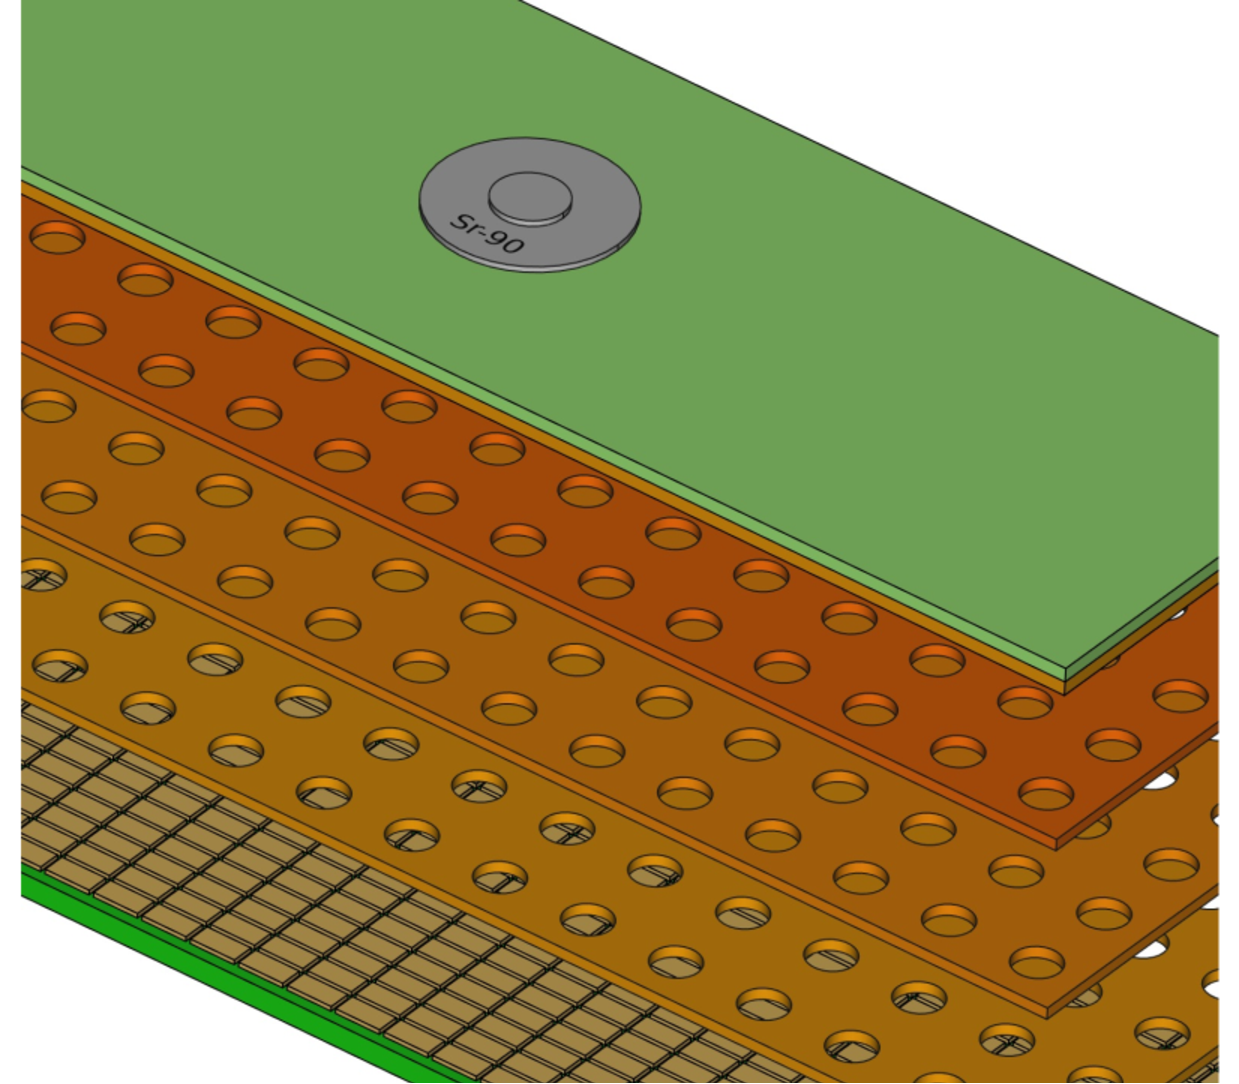
\includegraphics[height = 4 cm, width= 5.8cm]{img/GEM_Sr_source.pdf}
	\caption{Расположение источника относительно ускоряющей структуры}
	\label{fig:det_scheme+sr90}
\end{figure}
Электроны из источника проникали в газовый объем детектора и теряли энергию посредством ионизации. 
Первичная ионизация из дрейфового промежутка попадала в ускоряющую структуру, где происходило образование электронных лавин. Затем они проходили через два транспортных промежутка между GEM--электродами и попадали в индукционный промежуток. Заряд электронных лавин регистрировался считывающей структурой. По рассчитанному выше значению первичной ионизации и среднему заряду кластера определялся коэффициент усиления детектора. Цель эксперимента: проверить зависимость коэффициента усиления от напряжения. Для корректно работающей усиливающей и считывающей систем данная зависимость должна быть иметь экспоненциальный рост с увеличением напряжения. Набор статистики проходил в 7 точках по напряжению на ускоряющей структуре: от 3100 до 3450 В.

\subsection{Обработка и анализ полученных данных}
Полученные сырые данные обрабатывались с использованием алгоритмов, описанных в пункте \ref{sec:event_analysis}. После этого для каждого набора событий были построены распределения по заряду в кластерах. Для нахождения наиболее вероятного значения заряда экспериментальные гистограммы подгонялись функцией Ландау. После перевода каналов АЦП в единицы заряда коэффициент усиления находился по формуле \ref{eq:ampl_k}. На Рис. \ref{fig:charge_landau} можно видеть распределения по заряду кластера для двух точек по напряжению. 
\begin{figure}[h]
\centering
\begin{subfigure}{.45\textwidth}
	\centering
	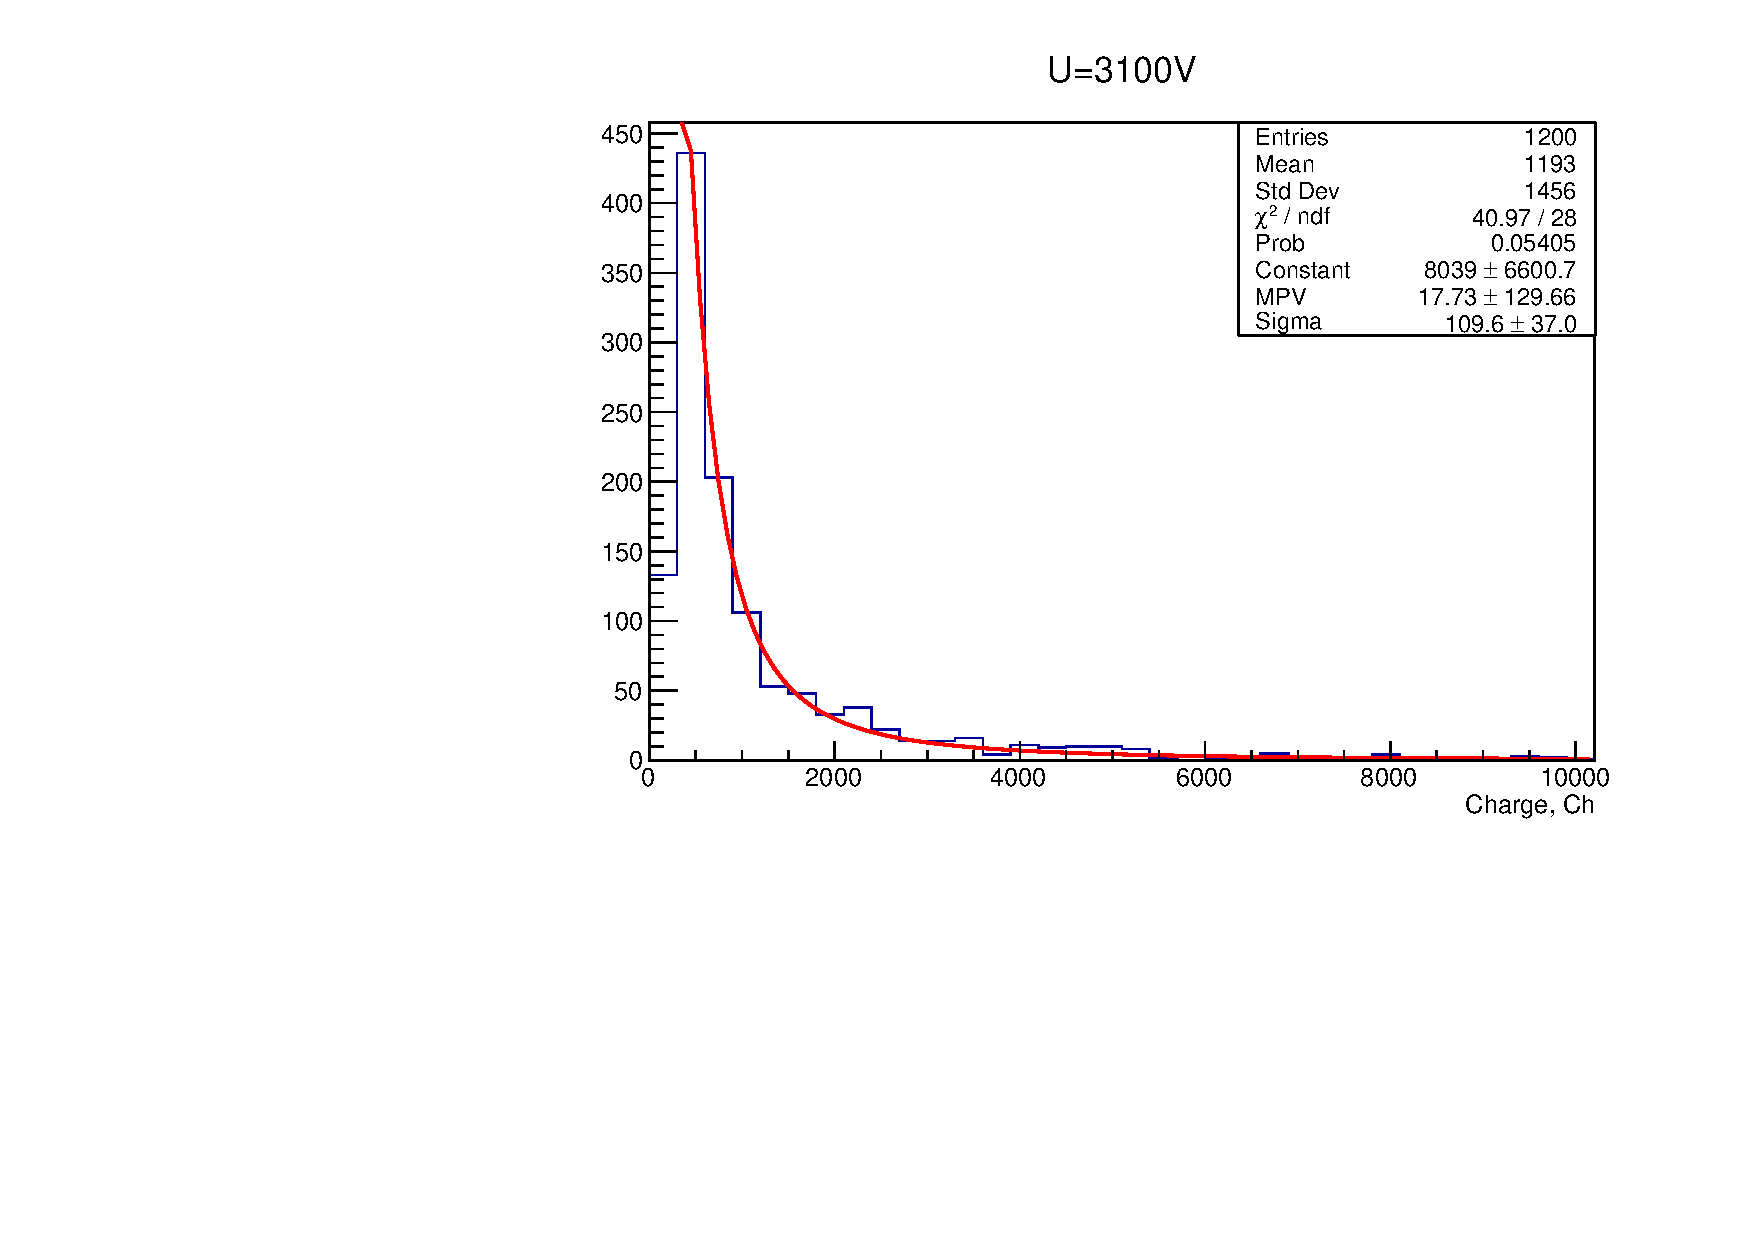
\includegraphics[width=1\linewidth]{img/3100.pdf}
	\caption{Напряжение на ускоряющей структуре 3100 В}
\end{subfigure}%
\hspace{20pt}
\begin{subfigure}{.45\textwidth}
	\centering
	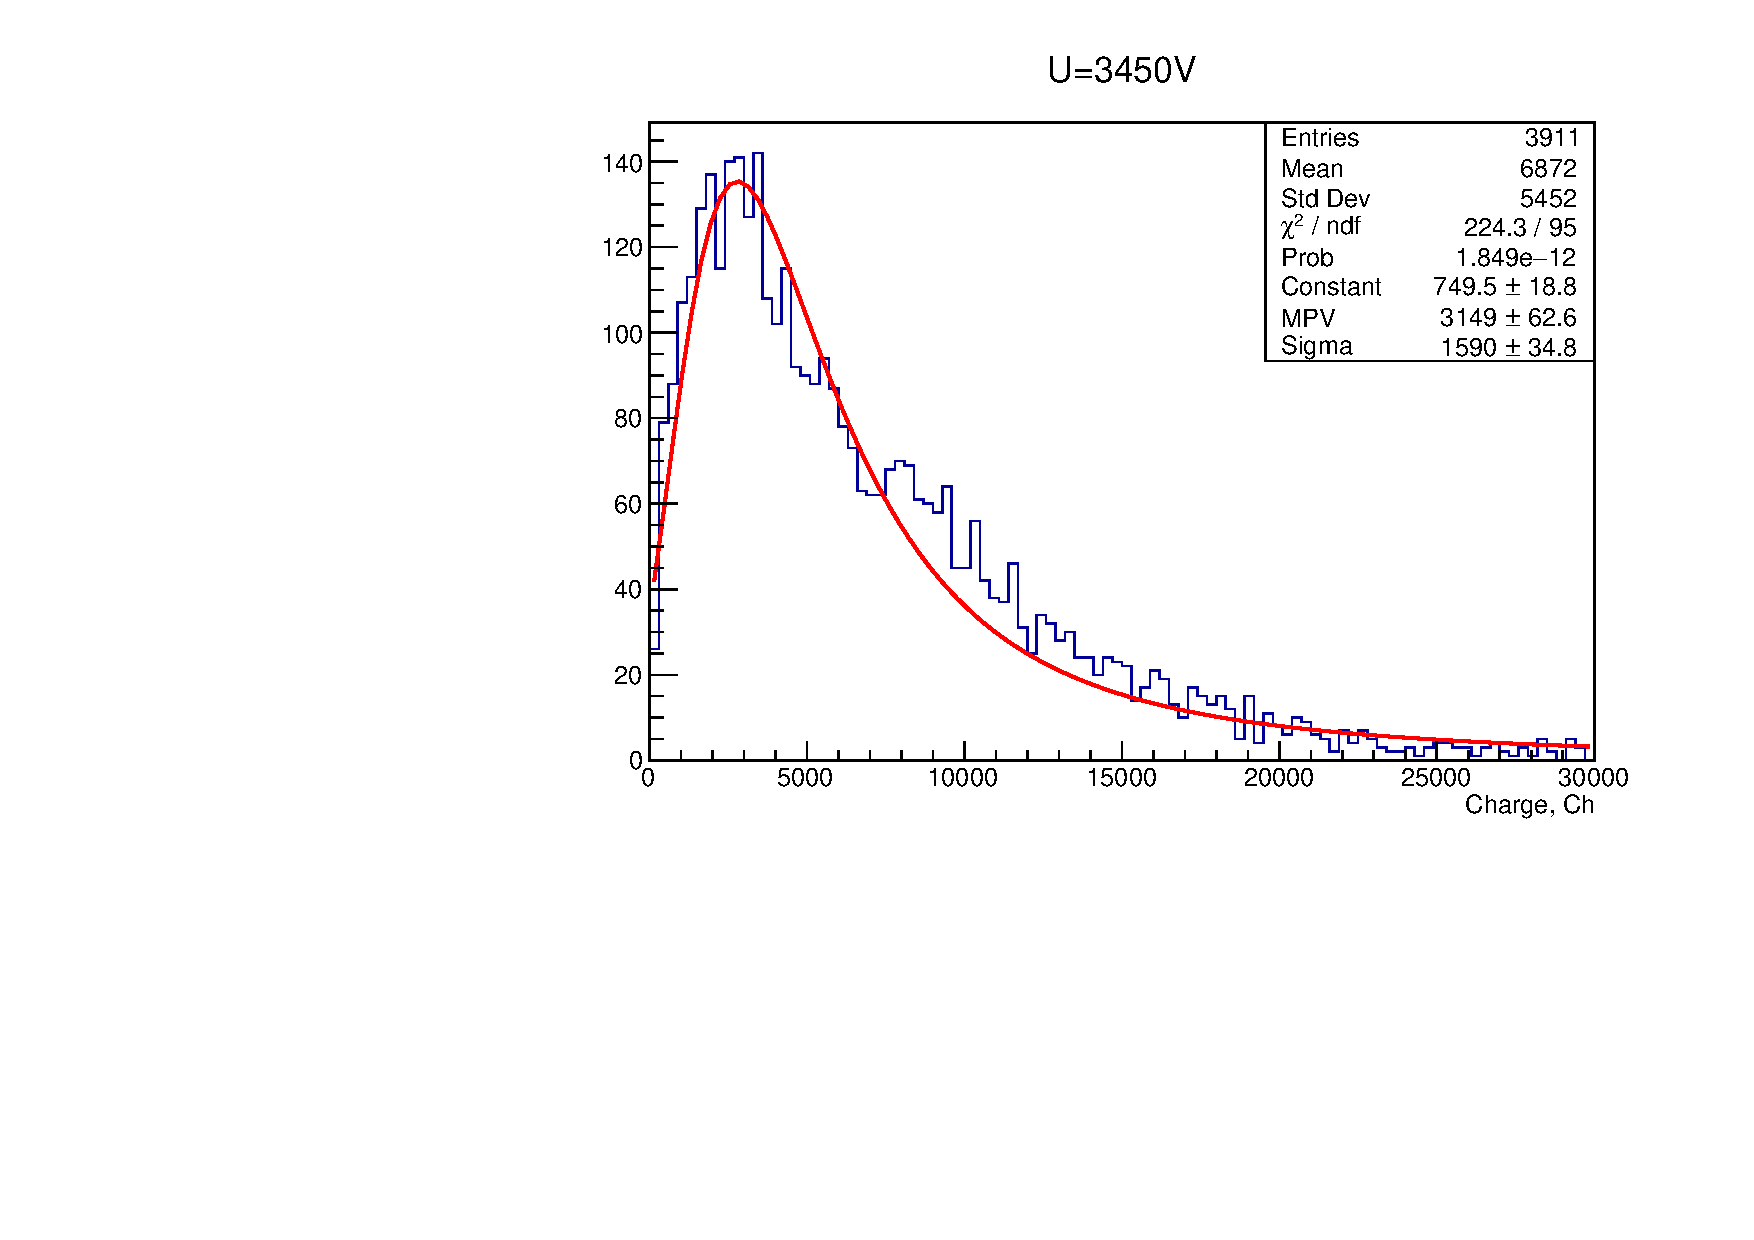
\includegraphics[width=1\linewidth]{img/3450.pdf}
	\caption{Напряжение на ускоряющей структуре 3450 В}
\end{subfigure}
\caption{Распределения по заряду кластера для разных значений напряжений на ускоряющей структуры детектора. Для напряжения 3100 В эффективность разделения сигнал--шум мала, поэтому положение пика распределения точно определить не получилось.}
\label{fig:charge_landau}
\end{figure}

\subsection{Результаты}
На Рис. \ref{fig:ampl_graph} представлены результаты измерений коэффициента усиления детектора. Для точек, где достоверно определен пик распределения Ландау наблюдается экспоненциальный тренд. Это указывает на правильную работу систем детектора.
\begin{figure}[h]
	\centering
	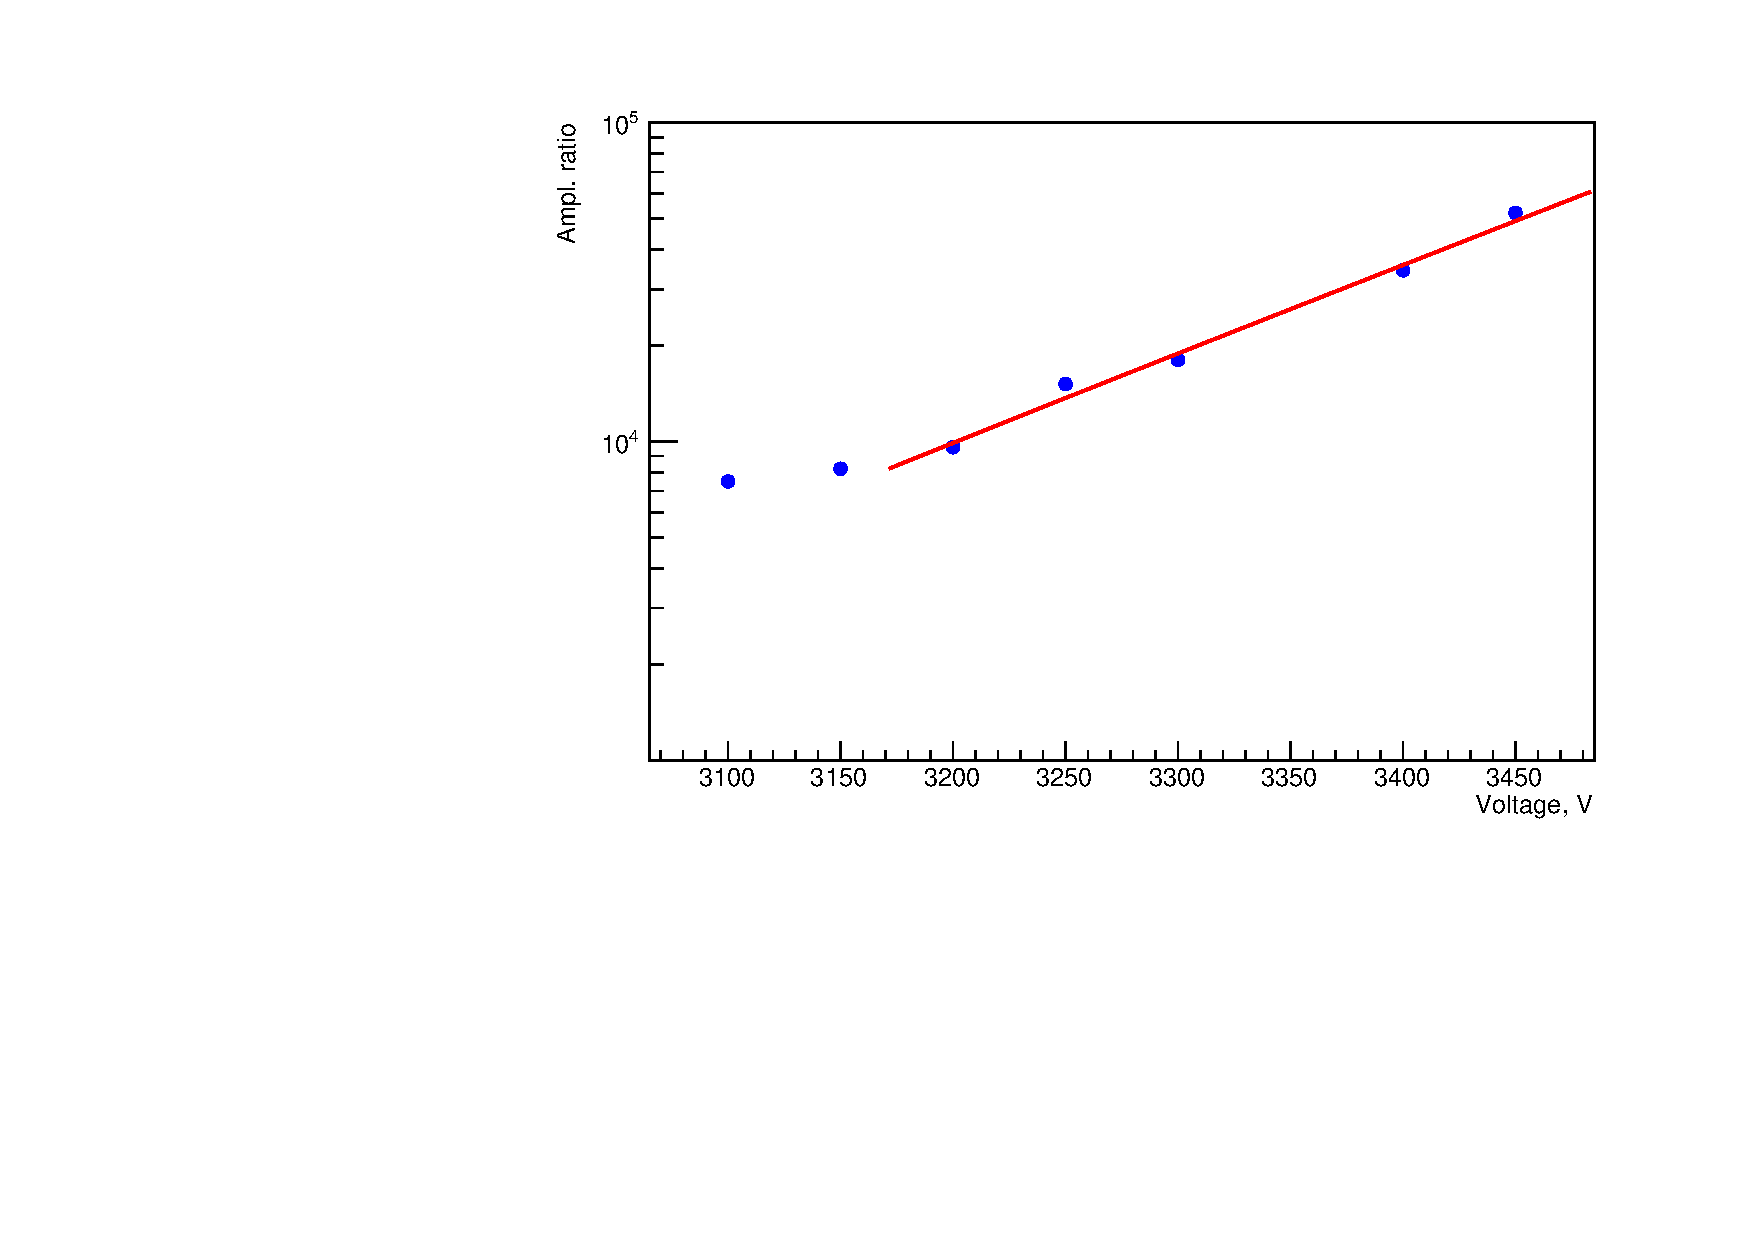
\includegraphics[width = 10cm]{img/Ampl_gr_log.pdf}
	\caption{Зависимость коэффициента усиления детектора от напряжения на ускоряющей структуре. Красная линия соответствует подгонке экспонентой.}
	\label{fig:ampl_graph}
\end{figure}
Максимальный коэффициент усиления, достигнутый при напряжении GEM--электродах 4500 В, составляет примерно 58000. Так же, при значении коэффициента усиления меньше 10000 достоверность разделения сигнала и шума резко уменьшается, что видно по количеству событий, отмеченных программой как сигнальные: при напряжении 3100 В было обработано 1200 сигнальных событий против 3900 при напряжении 3450 В. В точках с напряжением 3100 и 3150 В пик распределения Ландау был под границей шумов, поэтому его положение определялось лишь по правому склону распределения. Этим вызвана ошибка определения среднего заряда кластера, что привело к выполаживанию графика коэффициента усиления.

\section{Определение эффективности регистрации}
Еще одним параметром, который является ключевым для детектора, работающего в установке <<Лазерный поляриметр>>, является эффективность регистрации -- отношение числа зарегистрированных событий к их полному числу. Рассмотрим классическую схему для определения эффективности регистрации детекторов, которая подробно описана например в \cite{grupen}. Пусть имеется три детектора: D1, D2 и D3 с эффективностями $\varepsilon_1, \varepsilon_2$ и $\varepsilon_3$ соответственно. Требуется найти эффективность регистрации одного из них (для определенности выберем D1). Всего частиц, регистрируемых детекторами, $N_0$. Детекторы D2 и D3 необходимо включить в схему совпадений,т.е. сигнал о зарегистрированной частице должен генерироваться только тогда, когда они сработали одновременно. Это необходимо для эффективной фильтрации шумовых срабатываний. Схема из двух детекторов сможет зарегистрировать лишь $N_{23}$ событий. В предположении того, что акты регистрации частицы в двух детекторах абсолютно независимы, можно выразить $N_{23}$ как: 
\begin{equation}
N_{23} = \varepsilon_2\varepsilon_3 N_0.
\end{equation}
Если теперь добавить к этой схеме третий детектор и подсчитывать события, которые дали сигнал одновременно в трех детекторах, то их число будет: 
\begin{equation}
N_{123} = \varepsilon_1\varepsilon_2 \varepsilon_3 N_0.
\end{equation}
Отсюда можно определить эффективность регистрации третьего детектора: 
\begin{equation}
\varepsilon_1 = \frac{N_{123}}{N_{23}}
\end{equation}
Таким образом, для определения $\varepsilon_1$ необходимо знать количества событий, регистрируемых двумя схемами совпадений, одна из которых включает два детектора, а другая -- все три. Данный метод является простым и надежным, но не учитывает геометрических параметров детекторов, что так же может сильно повлиять на определяемое значение $\varepsilon$.
\subsection{Постановка эксперимента}
Измерение эффективности регистрации детектора <<Лазерного поляриметра>> было проведено на выведенном пучке электронов ускорителя ВЭПП-4М. Сначала был получен пучок тормозных гамма--квантов, которые затем конвертировались на свинцовой мишени в электрон--позитронные пары. Затем происходил отбор электронов по энергии с помощью спектрометрического магнита, за которым располагались детектирующая система.
 \begin{figure}[h]
 	\centering
 	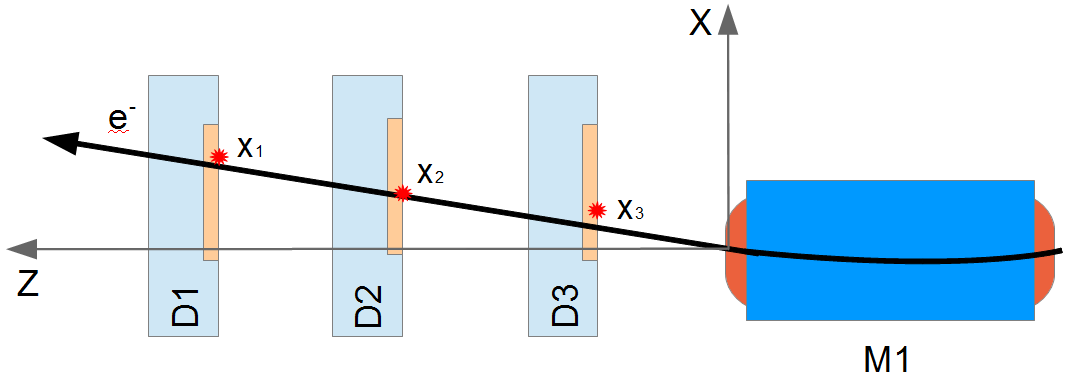
\includegraphics[width= 12cm]{img/reg_eff_exp_scheme.png}
 	\caption{Принципиальная схема установки для определения эффективности регистрации и пространственного разрешения на выведенном пучке ускорителя ВЭПП-4М. М1 -- спектрометрический магнит, D2,D3 -- вспомогательные детекторы, D1 -- исследуемый детектор.}
 	\label{fig:test_beam_scheme}
 \end{figure}
Для реализации схем совпадений помимо исследуемого детектора были использованы ещё два, которые работают в составе установки <<ДЕЙТОН>>. Это двухкоординатные GEM--детекторы с размером чувствительной области $160 \times 40$\,мм, применяемые на установке <<ДЕЙТОН>>. Все элементы схемы были позиционированы с помощью лазерных уровней и подключены к системе сбора данных выведенного пучка для того, чтобы получать сигналы триггера, который расположен сразу после мишени--конвертера. В ходе эксперимента тремя детекторами регистрировались координаты электронов выведенного пучка. Измерения проводились, начиная с напряжения на ускоряющей структуре 3200 В в шести точках с шагом 50 В. При последующей работе с данными события из разных детекторов связывались с помощью их порядкового номера в файлах. Стоит отметить, что данные, полученные при работе на выведенном пучке, были так же использованы для определения пространственного разрешения детектора. 

\subsection{Обработка и анализ полученных данных}
Сырые данные с детекторы были конвертированы в деревья (ROOT TTree). Каждое дерево содержало три ветви: две координаты и номер события. Для определения координат зарегистрированных частиц был программно реализован метод нахождения центра тяжести кластера. Его суть заключается в следующем: сначала определяются каналы, сигнал в которых превышает шумовой, затем по горизонтальной и вертикальной координате производится независимое суммирование вида: 
\begin{equation}
 \langle x \rangle = \frac{\sum_{i}q_i x_i}{\sum_{i}q_i},
\end{equation}
где $q_i$ -- заряд канала с координатой $x_i$. Нормировка производилось на полный заряд кластера.
\par По причине того, что чувствительная область детектора для поляриметра не охватывала весь пучок, стандартный алгоритм вычисления эффективности регистрации был модифицирован: в него добавлен учет геометрических параметров детектора и их влияние на конечную величину эффективности. Ниже приведена последовательность операций с данными для данного алгоритма.
\begin{itemize}
	\item Сначала отбирались события, попавшие в центральную область детектора <<Лазерного поляриметра>>
	\item Затем для этой выборки находились средние значения координат и дисперсии в дополнительных детекторах D2 и D3. 
	\item В детекторах D2 и D3 выделялись области с центром в точках, соответствующих средним значениям по выборке и размером в одно стандартное отклонение. 
	\item После этого \textit {по всему набору} подсчитывались события, которые попадают в выделенные области (в том числе и незарегистрированные исследуемым детектором.)
	\item Отношение числа событий из центральной области детектора <<Лазерного поляриметра>> к числу событий из выделенных областей дополнительных детекторов  регистрации. 
\end{itemize}
Используя данный алгоритм, удалось сделать поправку на неполное покрытие поперечного сечения пучка чувствительной областью детектора.
В ходе эксперимента измерена эффективность регистрации в шести точках по напряжению. Рис. \ref{fig:eff_gr} показывает, что при повышении напряжения питания ускоряющей структуры эффективность регистрации тоже возрастает. Максимально достигнутое значение эффективности регистрации $96 \pm 1\%$. 
\begin{figure}[h]
	\centering
	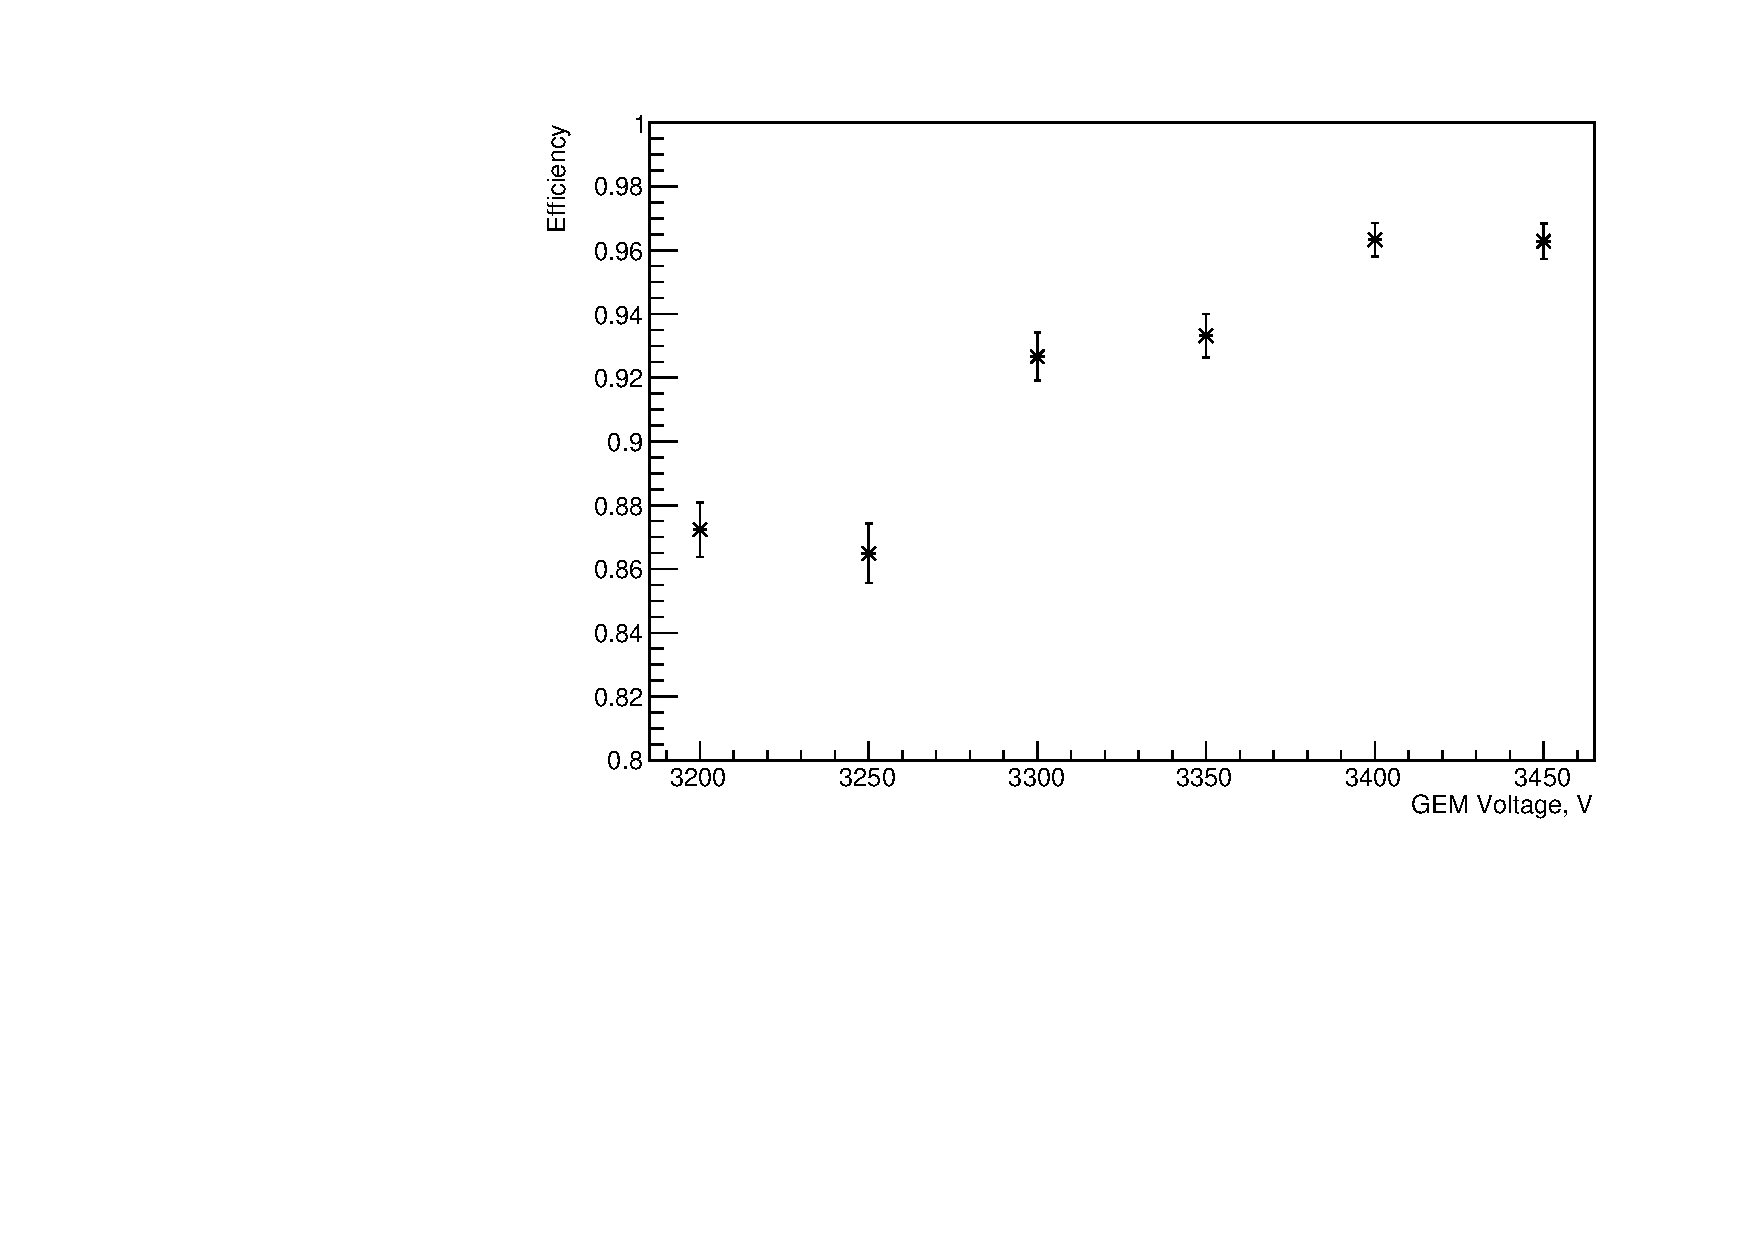
\includegraphics[width= 12cm]{img/eff_plot.pdf}
	\caption{Зависимость эффективности регистрации от напряжения на ускоряющей структуре.}
	\label{fig:eff_gr}
\end{figure}
Несмотря на то, что измерение и проводилось в центральной области детектора, где корректно работали практически все каналы, в отбор попали как минимум некорректно работающих 2 канала, которые программно отключались на этапе предобработки и вычитания пьедесталов. Поэтому реальное значение эффективности регистрации может быть выше. Тем не менее, результат эксперимента тоже является допустимым для прототипа детектора.  

\section{Определение пространственного разрешения}
В процессе измерения энергии детектор  <<Лазерного поляриметра>> должен достоверно разделять по координате два распределения фотонов разных поляризаций. Для этого нужно иметь сведения о пространственном разрешении детектора. Измерить пространственное разрешение можно следующим образом: пусть имеются данные о координатах частицы, прошедшей через все три детектора. Т.к. они находятся в области, где отсутствуют электрические и магнитные поля, то траектория частицы должна быть прямой. Полями в детекторах можно пренебречь т.к. пучок проходит почти перпендикулярно к главным плоскостям детекторов. Пусть в схеме на Рис. \ref{fig:test_beam_scheme} расстояния между детекторами по координате $z$ равны $z_{12}$ и $z_{23}$. Зная координаты частицы в третьем и втором детекторах, можно экстраполировать прямую, построенную по этим двум точкам в область, где находится детектор D1: 
\begin{equation}
	x_{1}^{*} = \frac{x_3- x_2}{z_{23}}(z_{12}+z_{23})+ x_3
\end{equation} 
Если теперь отнять это значение от измеренной координаты $x1$, то разница даст ошибку измерения  в первом детекторе. За пространственное разрешение принято брать корень из дисперсии распределения ошибок определения координаты. Данный метод справедлив при условии того, что источник частиц точечный, а координаты в двух дополнительных детекторах определяются точнее, чем в исследуемом. Тогда ширина распределения ошибок определяется именно пространственным разрешением тестового детектора.
\par В реальном же эксперименте размеры пучка составляют примерно $30\times 20$\,мм. Поэтому необходимо выделять коллинеарные треки, идущие с небольшой области, где наблюдается максимальная интенсивность. Также существует проблема смещения детекторов друг относительно друга, так, что их нулевые координаты не совпадают. Тогда за абсолютную координату можно взять значение в детекторе D3,а сдвиги нуля в двух других детекторах ($\Delta x_{23}$ и $\Delta x_{13}$) определить по средним значениям распределений величин $(x_2 - x_3)$ и $(x_1 - x_3)$. В конечном итоге формула для определения экстраполированной координаты $	x_{1}^{*}$ будет иметь вид: 
\begin{equation}
x_{1}^{*} = \frac{x_3- (x_2 -\Delta x_{23}) }{z_{23}}(z_{12}+z_{23})+ x_3 + \Delta x_{13}
\end{equation} 

\subsection{Обработка и анализ полученных данных}
Для определения пространственного разрешения были использованы данные, набранные на выведенном пучке и преобразованные в деревья, как описано выше. 
\begin{figure}[h]
	\centering
	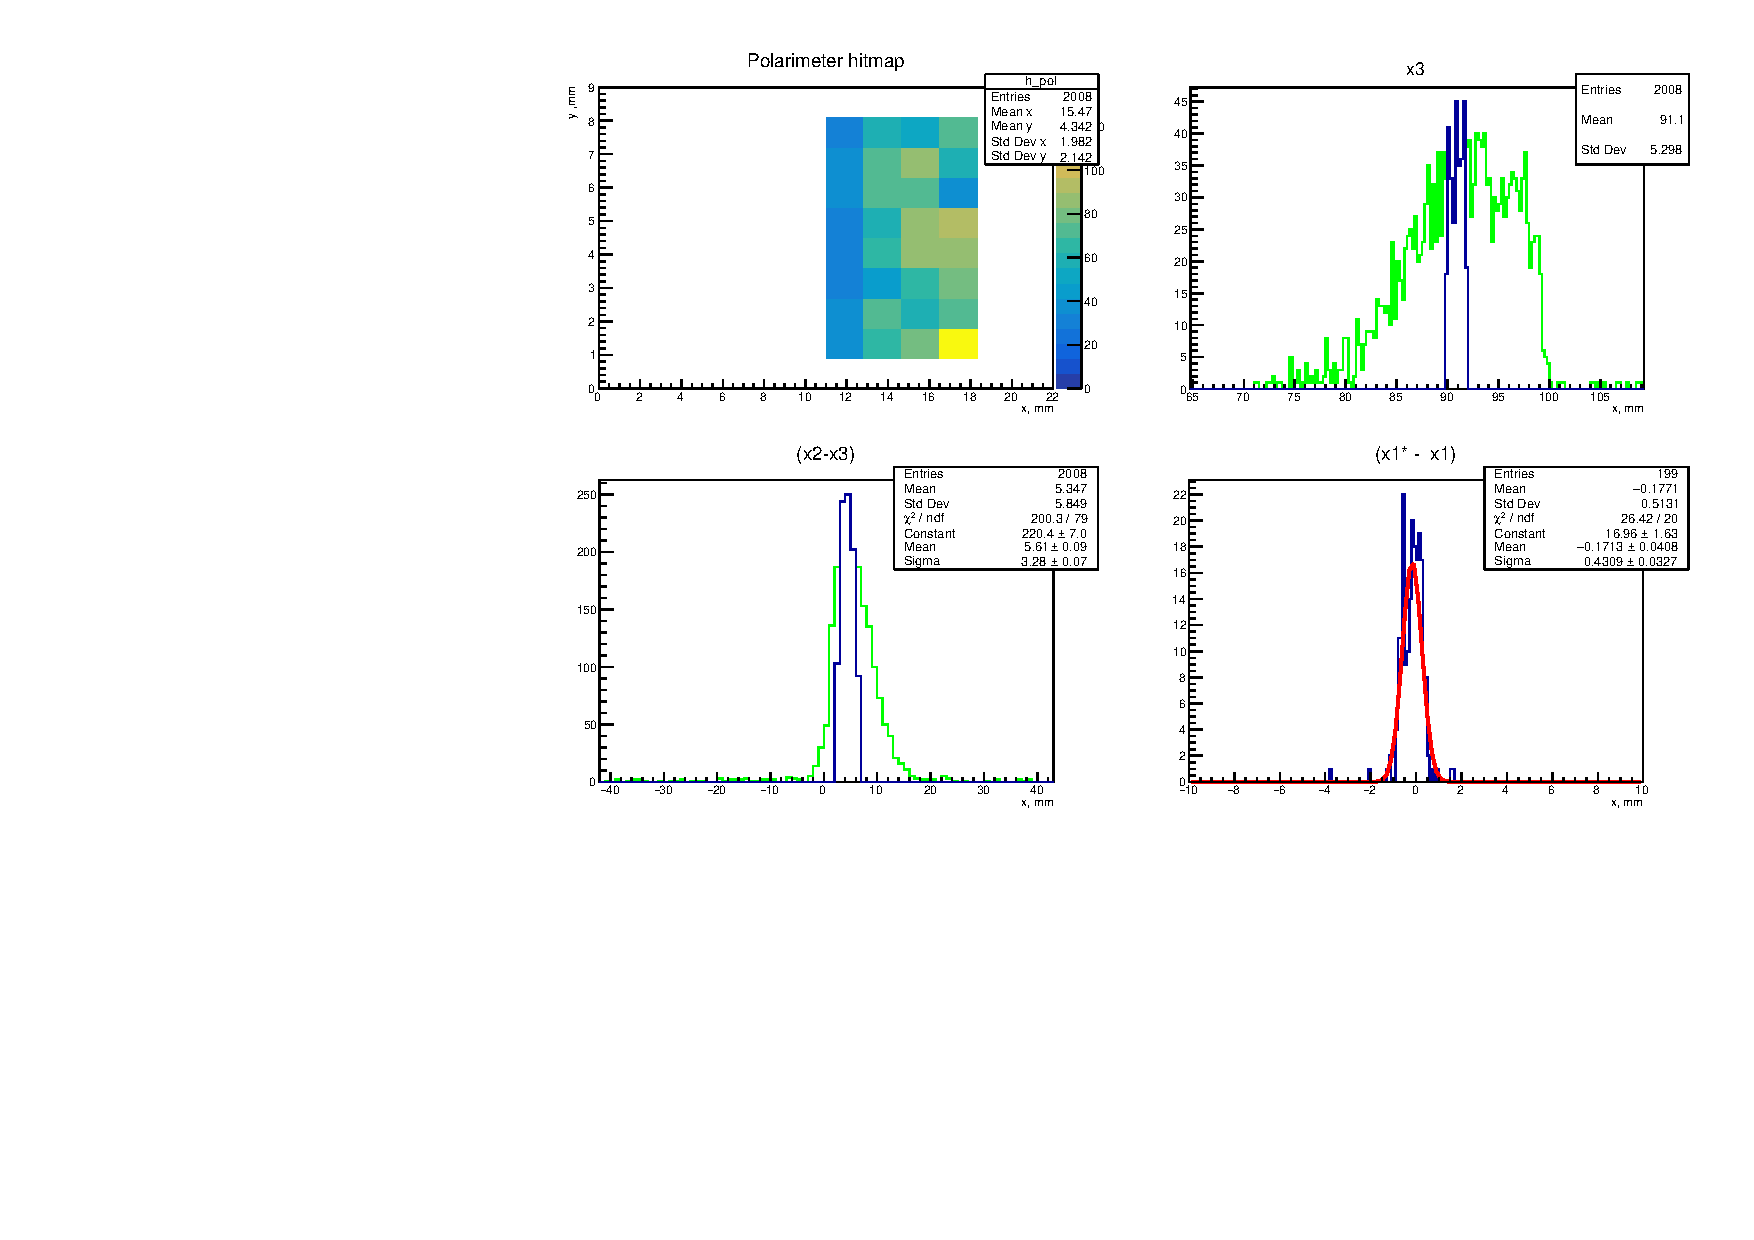
\includegraphics[width= 16cm]{img/sp_res_monitor.pdf}
	\caption{Монитор промежуточных результатов программы для вычисления пространственного разрешения детектора.}		
	\label{fig:sp_res_monitor}
\end{figure}

\subsection{Результаты}
\begin{figure}[h]
	\centering
	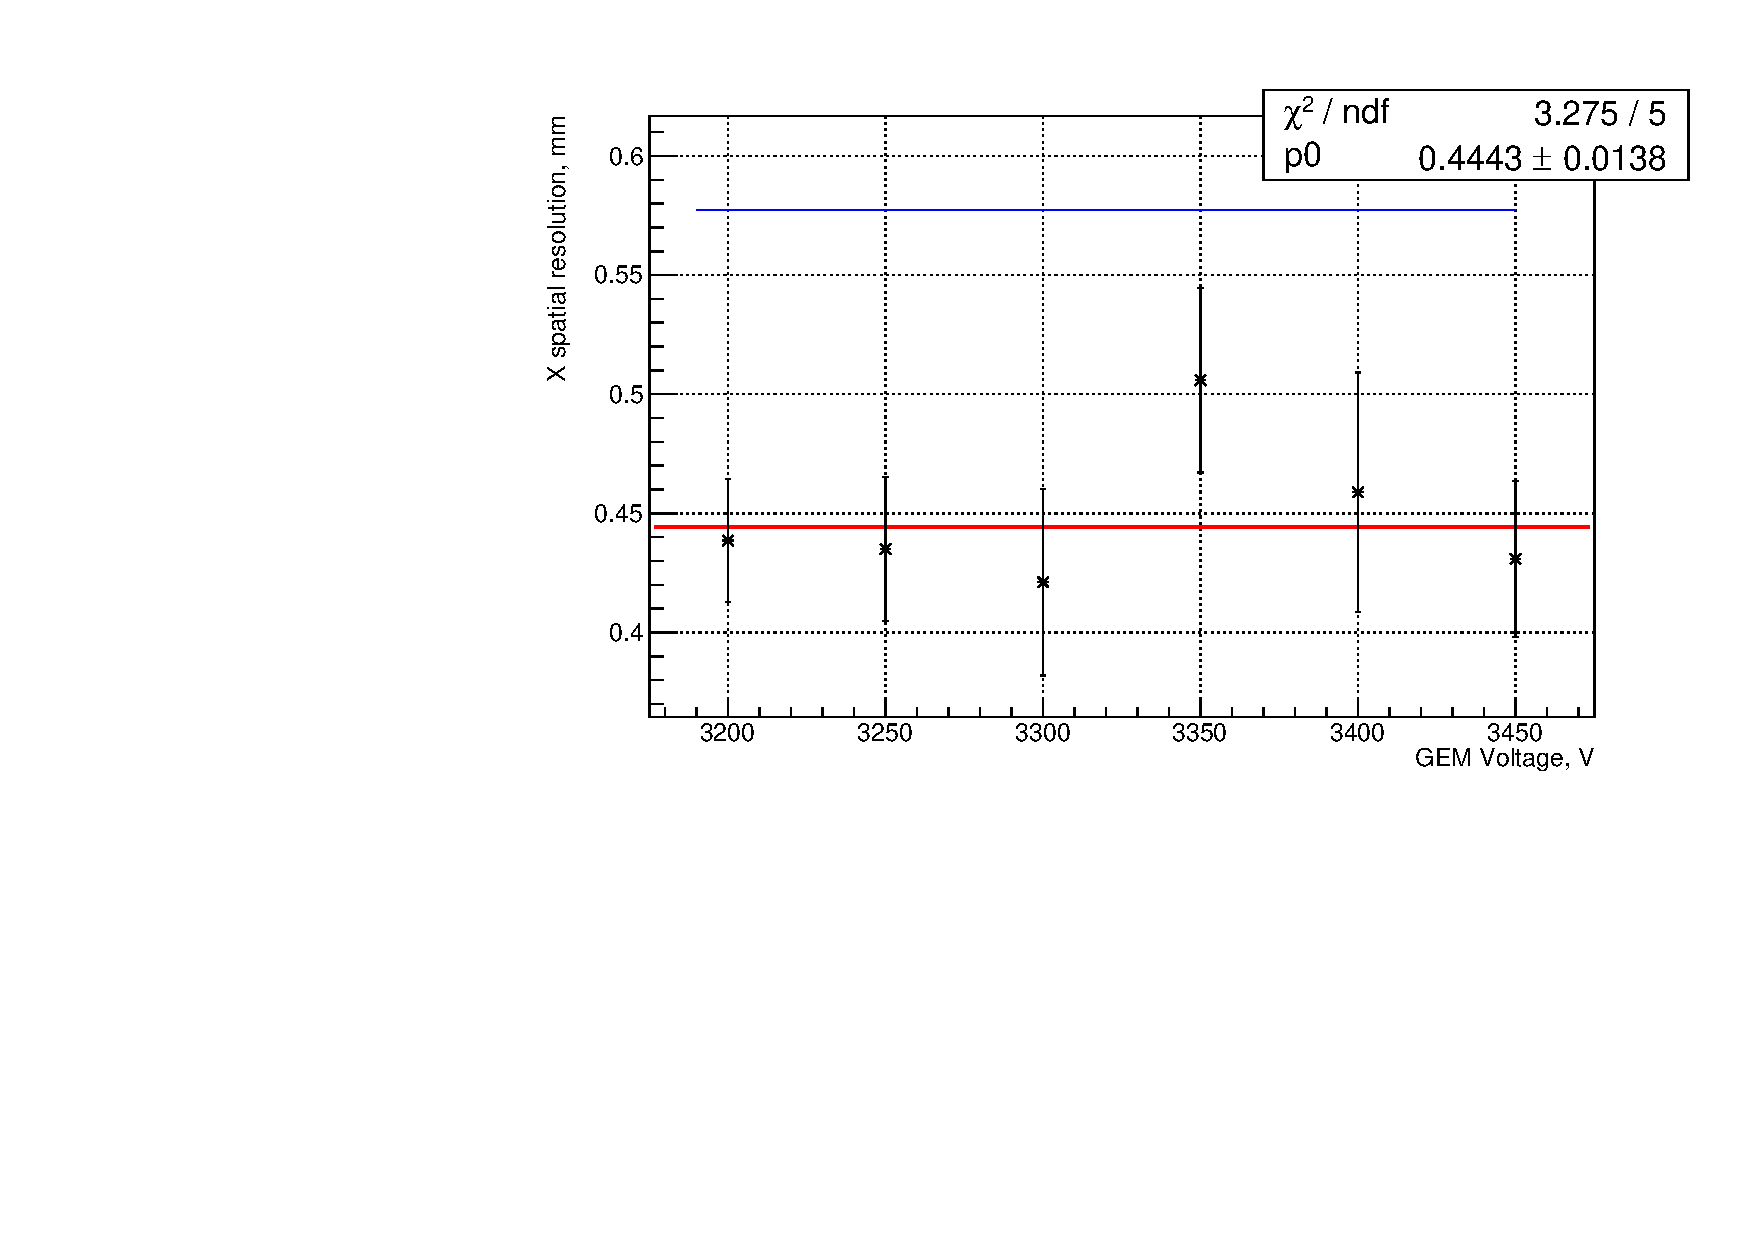
\includegraphics[width= 12cm]{img/x_sp_res.pdf}
	\caption{Пространственное разрешение по вертикальной координате. Синяя линия -- теоретическое предсказание в случае работы в режиме идентификации. Красная линия -- результат аппроксимации данных функцией $y = const$.}
	\label{fig:x_sp_res}
\end{figure}

\begin{figure}[h]
	\centering
	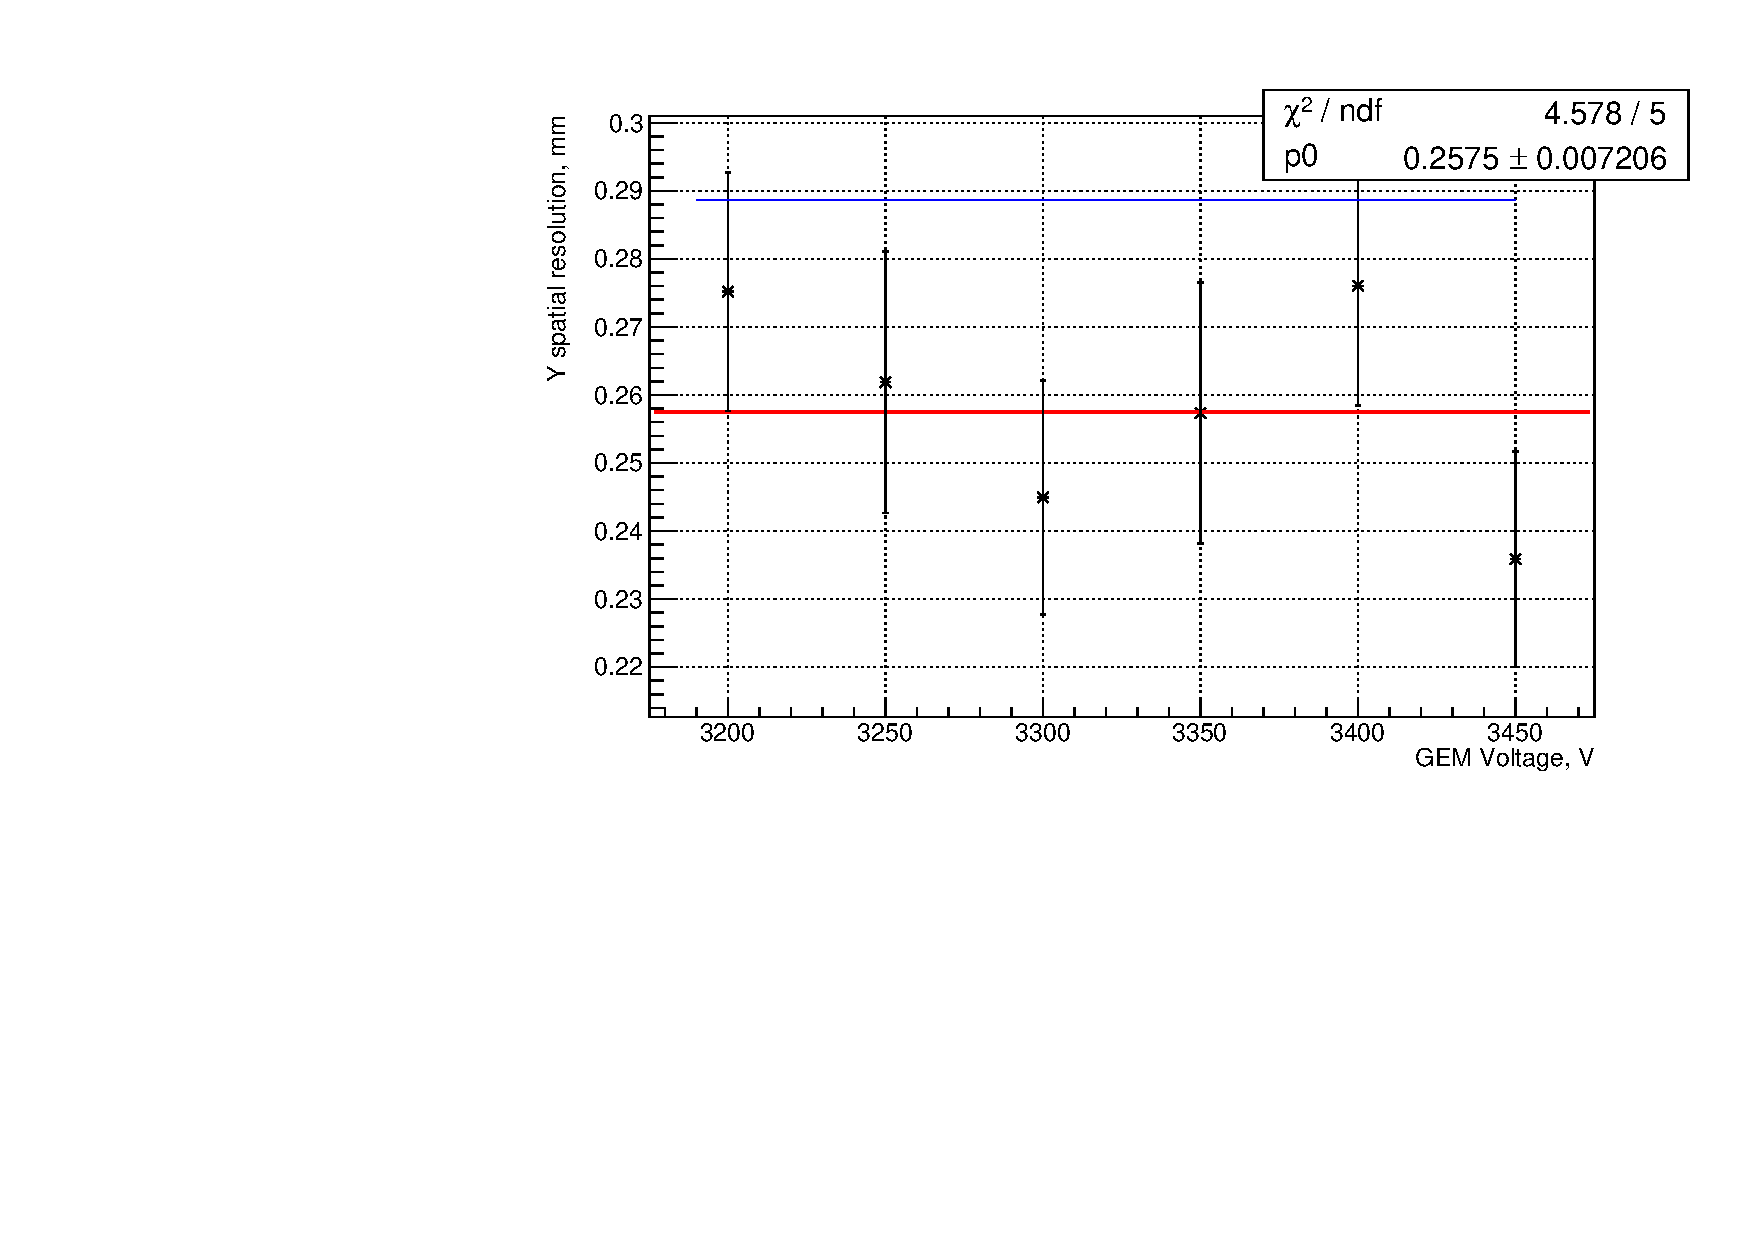
\includegraphics[width= 12cm]{img/y_sp_res.pdf}
	\caption{Пространственное разрешение по вертикальной координате. Синяя линия -- теоретическое предсказание в случае работы в режиме идентификации. Краснаяя линия -- результат аппроксимации данных константой.}
	\label{fig:y_sp_res}
\end{figure}